\documentclass[/home/greg/Thesis/main/main.tex]{subfiles}

\begin{document}
\graphicspath{{/home/greg/Neutron_star_modelling/TwoStateSwitching/PrecessionInducedBySwitching/img/}}

\section{Precession induced by torque switching}

Damping mechanisms in NSs (which are supported by the observation of exponential
recovery from glitches) indicate that NS will not precess. This means that general
solutions should assume their spin axis is aligned with the body frame. However, 
as we have already shown (3.4 of transfer thesis) the anomalous component of the
\citet{Deutsch1955} torque modifies the body frame: stable, non-precessing solutions
correspond to those aligned with the effective body frame axis. This effective
body frame, denoted by $[\1, \2, \3]$, corresponds to a rotation of the original
body frame ($[\x, \y, \z]$) by an angle~$\beta$
\begin{align}
    \left[\begin{array}{c} \1 \\ \2 \\ \3 \end{array} \right] = 
    \left[\begin{array}{ccc} 
            \cos(\beta) & 0 & \sin(\beta)  \\
            0 & 1 & 0  \\
            -\sin(\beta) & 0 & \cos(\beta)  
    \end{array} \right]
    \left[\begin{array}{c} \x \\ \y \\ \z \end{array} \right].
\end{align}
The rotation angle is given by 
\begin{equation}
    \beta(\epsI, \epsA, \chi) = \arctan\left(
    \frac{\epsI - \epsA \cos(2\chi) - \sqrt{\epsI^{2} + \epsA^{2} -2\epsA\epsI\cos(2\chi)}}
    {2\epsA\sin(\chi)\cos(\chi)}
    \right).
\end{equation}
So we should expect steady, non-precessing NS to make an angle $\beta$ with 
the $\z$ or $\x$ axis corresponding to alignment with the body frame axis.

For the two-state switching model proposed by \citet{Lyne2010} to explain 
timing noise in pulsars, pulsars undergo switching between two distinct spin-down
values. Physically this must correspond to a change in the dipole moment of
the spin-down torque. In our model the strength of the torque is parameterised
by $\epsA$, related to the surface magnetic field strength by 
\begin{align}
    \epsA = \frac{R^{5}}{4I_{0} c^{2}} B_{0}^{2}.
\end{align}
Rearranging equation (1.4.8) of my transfer thesis we can then write the 
spindown as 
\begin{align}
    \dot{\omega}_{0} & = -\frac{B_{0}^{2}R^{6} \sin^{2}(\alpha) \omega_{0}^{3}}{6 I_{0} c^{3}} \\
    & = - \frac{2 R \epsA \sin^{2}(\alpha) \omega_{0}^{3}}{3 c}.
\end{align}
Recalling that $\alpha$ is the angle between the rotation axis and magnetic dipole
this term is approximately unity. Taking the spin frequency as a fixed value yeilds
and estimate for the spin-down frequency
\begin{equation}
    \fdot = - \frac{R \epsA  \omega_{0}^{3}}{3\pi c}.
    \label{eqn: spin-down of epsA}
\end{equation}

If, in the two-state switching model, the spin-down value changes by a fraction
$\upsilon$ such that
\begin{equation}
    \fdot \rightarrow \fdot' = (1-\upsilon)\fdot,
\end{equation}
then from equation \eqref{eqn: spin-down of epsA} 
\begin{equation}
    \epsA \rightarrow \epsA' = (1-\upsilon)\epsA.
\end{equation}

The two-state switching changes the value of $\epsA$ and so has a knock-on 
effect on the effective body frame. A non-precessing NS at an
angle $\beta(\epsI, \epsA, \chi)$ will, after a torque switch by a fractional
amount $\upsilon$, no longer be aligned with the body frame axis. This is 
because the effective body frame will have shifted to 
$\beta' = \beta(\epsI, \upsilon\epsA, \chi)$. As a result, we should expect the
previously non-precessing NS to begin precessing after a torque switching event. 

The NS will precess at the usual precession frequency in a cone  of half-angle
$\Delta\beta(\epsI, \epsA, \chi, \upsilon)=|\beta - \beta'|$ about the new
effective body-frame axis.  The expression for $\Delta \beta$ is not amenable
to manipulation but can easily be explored graphically. This is done in figure
\ref{fig: DeltaBetaPlot} for several choices of $\upsilon$. This illustrates
that the precession angle can be as much as a few degrees although it tends to
zero in the limit $\epsI \gg \epsA$.

\begin{figure}
    \centering
    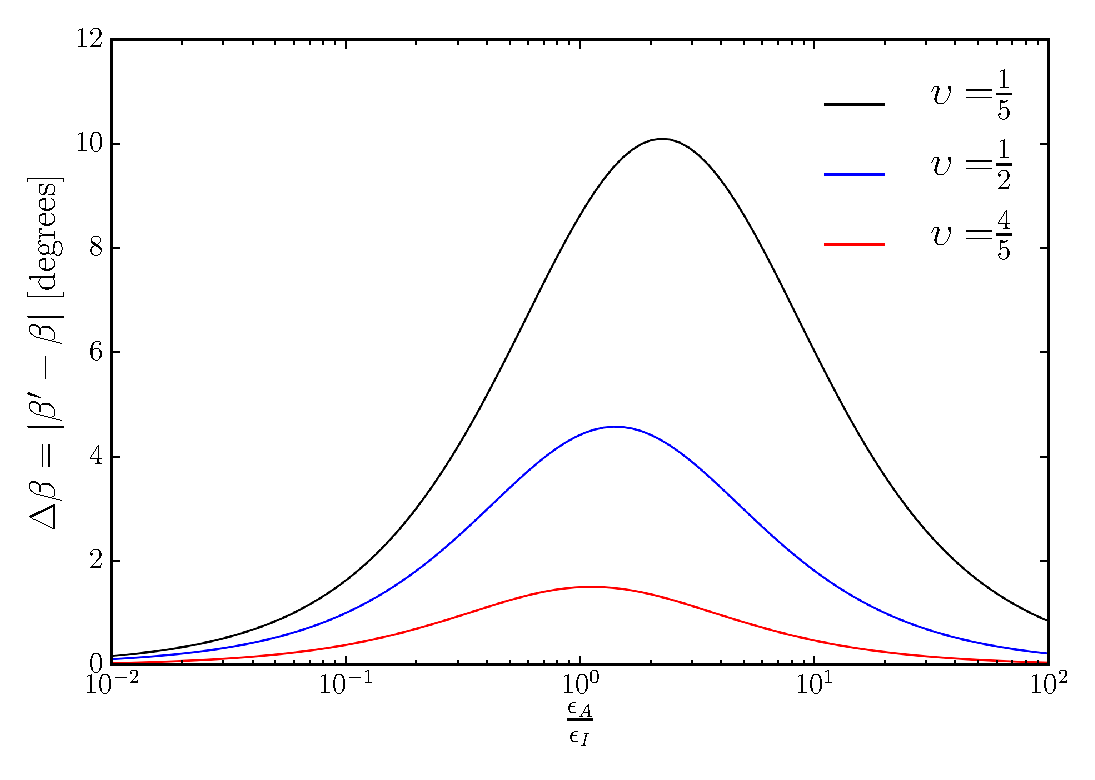
\includegraphics[width=0.5\textwidth]{DeltaBetaPlot}
    \caption{Illustrating the magnitude of the precession angle after switching
        due to the new rotation of the effect body frame. We plot the half-angle
        ($\Delta\beta$) of the precession cone as a function of the ratio
    $\epsA/\epsI$. Typically we expect real stars to have $\epsA < \epsI$.}
    \label{fig: DeltaBetaPlot}
\end{figure}

Since it is hard to gauge the significance of this we will apply it to the
PSR B1828-11; a pulsar which demonstrated evidence for precession \citet{Stairs2000}
and has since been reinterpreted as two-state switching \citep{Lyne2010}. This
has a frequency of $\f = 2.47$~Hz, a spin-down $\fdot=-3.65\times10^{-13}$~Hz/s, switches are
observed to occur every $T\approx 1.4$ yrs, and the spindown changes by $\upsilon = 0.71$.

We are unable to directly calculate $\Delta\beta$ from this information, since
we do now know $\epsI$ or $\chi$. Nevertheless, we can at least find the maximum
allowed value found when $\chi \ll 1$ and $\epsI \sim \epsA$. This has not 
been found exactly although it could easily be done by maximising the function 
numerically. Approximately the maximum allowed angle is $\Delta\beta \sim 45^{\circ}$.

We can now attempt to quantify the effect this may have on the timing residuals.
Precession, as shown by \citet{Jones2001}, will produce a sinusoidal variation
in the residual with a magnitude given by 
\begin{equation}
    \Delta\Phi_{\mathrm{FP}} \sim \pi \cot(\chi) \theta.
\end{equation}
This precession will be damped by other processes, but in the immediate aftermath
of a switch, may be detectable. 

However, when considering the residual which includes a switch we must also
take into acount the effect this will have. This was considered in section (6.6)
of my transfer thesis. Here we present the result that, the maximal size of phase-residuals
assuming several switched occur during an observation is given by 
\begin{equation}
    \Delta\Phi_{\mathrm{TS}} \sim \frac{\pi}{16} \upsilon \fdot  T^{2},
\end{equation}
Where $T$ is the switching period

For PSR B1828-11 then we can directly compute the magnitude of variations in
the timing residual:
\begin{align}
    \Delta\Phi_{\mathrm{TS}}^{\mathrm{B1828-11}}= 95\mathrm{~s}
\end{align}
This is considerably larger than the result from \citet{Lyne2010} who measured a 
peak to peak residual of 94 ms.


\biblio
\end{document}

